\documentclass{article}
\usepackage{ctex}
\usepackage[a4paper]{geometry}
\usepackage{graphicx}
\usepackage{float}
\usepackage{xcolor}
\title{Chap1 超标量处理器概览}
\author{}
\date{}
\geometry{left=2cm, right=2cm, top=2cm, bottom=3cm}

\begin{document}
  \maketitle
  \section{为什么需要超标量}
  计算机领域有一个经典的公式来描述程序执行的时间,即:
  $${Total Instructions} \times \frac{Cycles}{{Instructions}} \times \frac{{Seconds}}{{Cycle}}$$
  
  第一项:总指令数。取决于:程序本身工作量、算法、编译器、指令集扩展(多媒体指令)等。

  第二项:即CPI(IPC的倒数)。对于普通流水线处理器,IPC最大为1,想要每周期执行多于一条指令,需要使用超标量处理器。
  并不是每周期执行的指令个数多于一条的处理器都是超标量处理器,VLIW结构处理器每周期也多于一条指令。

  第三项:周期时间(处理器主频的倒数)。取决于:电路设计、流水线级数、工艺。

  程序一定的情况下,IPC越大、主频越大,执行越快。但是IPC和主频互相制约。更深流水线的小周期处理器在
  预测失败时有更大的惩罚,反面教材:Intel的Pentium4系列处理器。
  
  超标量处理器每周期可以从I-Cache中取出n条指令送到流水线中,每周期内最少可以同时执行n条指令,称为n-way的超标量处理器。
  超标量与VLIW的区别:超标量处理器靠硬件自身决定哪些指令可以并行执行,VLIW依靠编译器和程序员自身。VLIW更多被使用在
  功能比较专一的处理器领域,例如DSP处理器。

  \section{普通处理器的流水线}
  \subsection{流水线概述}
  流水线可以降低处理器周期时间、获得更快的频率。

  当处理器没有流水线时,周期时间为$D$,频率为$1/D$;使用$n$级流水线后,周期时间变为$D/n+S$,
  频率变为$1/(D/n+S)$,$S$为流水线寄存器延迟。当没有使用流水线时,消耗硬件面积为$G$;使用了
  $n$级流水线后,消耗的硬件面积为$G+n\times L$。我们考虑消耗面积与频率的乘积,即$(G+n\times L)/(1/(D/n+S))=GD/N+SL\times n+LD+GS$。
  可以发现$n=\sqrt{GD/LS}$时即为最优化的流水线级数$n$(理论值)。

  \subsection{流水线的划分}

  流水级的划分应该满足以下条件。

  1.流水线中每个阶段所需要的时间是近似相等的,最长的流水段所需要的时间决定了整个处理器的周期时间。

  2.流水线中每个阶段的操作都会被重复地执行。

  3.流水线中每个阶段的操作都和其他流水段相互独立、互不相干。

  典型的RISC五级流水:取指、译码、执行、访存、写回。

  如何对流水线各个阶段进行平衡?

  方法一:将两个或多个流水段合并成一个流水段,但是现代高性能处理器都追求比较高的运行频率。

  方法二:将流水线的一个阶段拆成多个更小的阶段,适合高性能处理器。

  \subsection{指令间的相关性}

  数据相关:RAW、WAR、WAW,控制相关。

  \section{超标量处理器的流水线}

  如果一个处理器每周期可以取出多于一条的指令送到流水线中执行,并且
  使用硬件来对指令进行调度,那么这个处理器可以称为超标量处理器。
  对于乱序执行的超标量处理器,只有Issue阶段和Write back阶段可以乱序,
  前端(取指、译码)和后端提交阶段只能顺序。Issue:指令送到对应的功能单元;
  Write back:将指令的结果写到目的寄存器中。

  \subsection{顺序执行}

  顺序执行的超标量处理器:
  \begin{figure}[H]
    \centering
    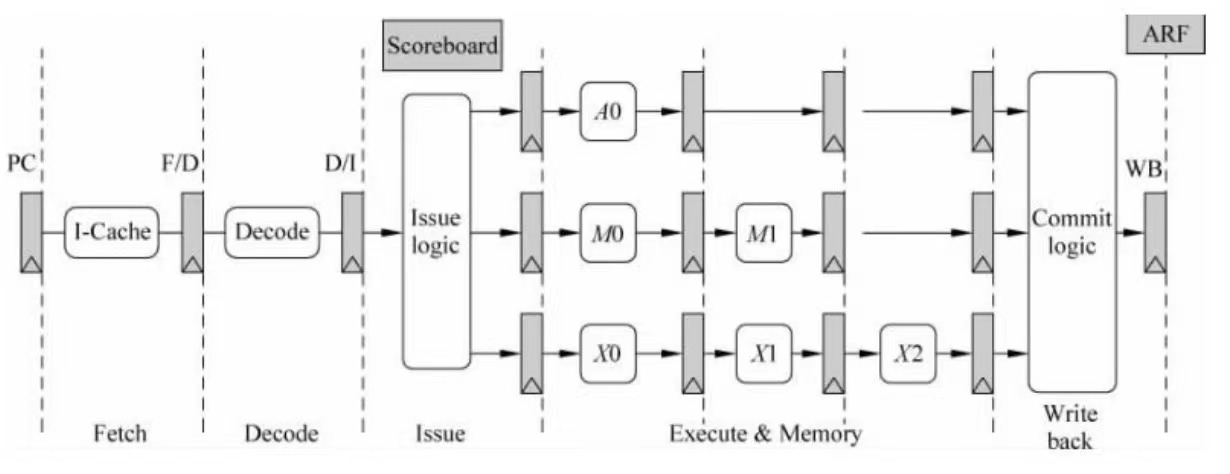
\includegraphics[width=14cm]{./figures/chap1_inorder_CPU.jpg}
  \end{figure}

  这个图里面没有考虑寄存器重命名。

  大体上直接都能看懂,指令解码之后根据自身类型送到对应的FU中执行,
  这个过程叫发射,单独一个流水级。
  
  ScoreBoard用于记录流水线中每条指令
  的执行情况,例如在哪个FU执行,什么时候可以计算出结果等。
  发射阶段把指令的信息写到ScoreBoard中,同时查询ScoreBoard获知
  自己的源操作数是否都准备好。


  \begin{figure}[H]
    \centering
    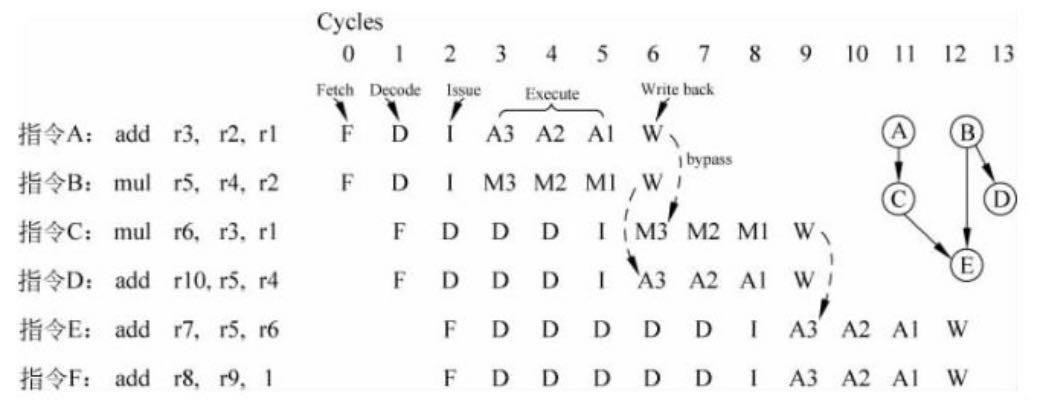
\includegraphics[width=13cm]{./figures/chap1_prog.jpg}
  \end{figure}

  
  上面是一段程序在上述处理器中的执行情况,右边描述了RAW相关的情况。
  可以看到只有数据准备好之后才会进入FU,否则一直停留在发射队列中。

  \textcolor{red}{个人认为这个图有错误,指令E和指令F在第3、4拍应该还是在F流水级
  ,不能进入D吧?}

  \subsection{乱序执行}

  一旦某条指令的操作数准备好了,就可以将其送到FU中执行。
  \begin{figure}[H]
    \centering
    \includegraphics*[width=14cm]{./figures/chap1_oor.jpg}
  \end{figure}

  为了在乱序执行时解决WAW和WAR两种相关性,需要对寄存器进行重命名,
  处理器中有物理寄存器堆(PRF),指令集中定义的是ARF逻辑寄存器堆。
  
  到发射阶段(Issue)之前都是顺序的,发射阶段有发射队列(Issue Queue, IQ),
  发射阶段是顺序到乱序的分界点。

  由于分支预测失败或者异常的存在,PRF的结果未必都会写到ARF中,因此PRF也成为Future File。
  为了保证程序的串行结果,指令需要按照程序中规定的顺序更新处理器状态,这需要使用重排序缓存(ROB)。
  流水线中所有的指令都按照程序中规定的顺序存储在重排序缓存中,使用重排序缓存实现
  对处理器状态的顺序更新,这个阶段称为提交阶段,在提交阶段结果从PRF写入到ARF中。如果不存在异常,
  指令可以顺利地离开流水线,并对处理器状态进行更改,称指令退休了。  一条指令在退休之前,都可以从流水线中被清除。

  对于store指令,防止写入内存后出现分支预测失败或者异常,使用Store Buffer,退休时才写入内存。

  \begin{figure}[H]
    \centering
    \includegraphics*[width=14cm]{./figures/chap1_oor_prog.jpg}
  \end{figure}

  需要注意的点:r表示算好了在ROB等待退休,提交是顺序的。

  ~\\

  超标量处理器流水线的各个阶段:

  1.Fetch:取指令并预测PC

  2.Decode

  3.Register Renaming:解决WAW和WAR两种伪相关性。

  4.Dispatch:在此阶段,被重命名后的指令写到发射队列、重排序缓存和Store Buffer等部件中。
  
  5.Issue:仲裁电路从IQ中挑选合适的指令送到FU中执行。发射队列中有唤醒电路,可以将
  发射队列中对应的源操作数置为有效状态。

  6.Register File Read:读PRF或者旁路。

  7.Execute

  8.Write back

  9.Commit:根据重排序缓存

\end{document}